\documentclass[aps,prb,onecolumn,superscriptaddress,nofootinbib,11pt]{revtex4-2}

\usepackage[utf8]{inputenc}
\usepackage[T1]{fontenc}
\usepackage{amsmath,amssymb,mathtools}
\usepackage{siunitx}
\usepackage{graphicx}
\graphicspath{{sections/}}
\usepackage{booktabs}
\usepackage{tikz}
\usetikzlibrary{arrows.meta, calc, positioning}
\usepackage{hyperref}

\newcommand{\ii}{\mathrm{i}}
\DeclareMathOperator{\Rey}{Re}
\DeclareMathOperator{\Imy}{Im}

\sisetup{range-phrase=--, range-units=single, detect-all}

% ------- unified layer-stack sketch ----------------------------------------
\tikzset{
  slab/.style   = {draw, thick, minimum width=5cm},
  ray/.style    = {-{Latex[length=1.6mm]}, thick, black},
  normalline/.style = {densely dashed, gray!70},
  anglearc/.style = {gray!80, thin},
  lbl/.style    = {font=\scriptsize},
}

\newcommand{\raysketch}[3]{%
  \pgfmathsetmacro{\xh}{#1}
  \pgfmathsetmacro{\thi}{#2}
  \pgfmathsetmacro{\dxi}{1.2*sin(\thi)}
  \pgfmathsetmacro{\dyi}{1.2*cos(\thi)}
  \draw[normalline] (\xh,-0.2) -- (\xh, 2.0);
  \draw[ray] (\xh-\dxi, \dyi) -- (\xh, 0);
  \draw[ray] (\xh, 0) -- (\xh+\dxi, \dyi);
  \draw[anglearc] (\xh, 0.7) arc [start angle=90, end angle=90-\thi, radius=0.7];
  \node[lbl, gray!90] at (\xh - 0.22, 0.95) {$\theta_0$};
}

\begin{document}

\title{Analytical benchmarks of the \texttt{tmm-core} package\\[2pt]
\large\normalfont Sixteen worked examples from first principles to ellipsometry}
\author{D.~Redka}
\affiliation{Laser Center HM, Munich University of Applied Sciences HM}
\date{\today}

\begin{abstract}
The sixteen worked examples collected below validate the transfer-matrix
method (TMM) implementation against closed-form analytical solutions
wherever such solutions exist. The ordering runs from the single planar
interface to absorbing multilayers and ellipsometric inversion, so that
each successive geometry introduces one additional ingredient of the
theory. Throughout, the code uses the sign convention in which $r_s = r_p$
at normal incidence; where a textbook formula is stated in the opposite
sign convention, the discrepancy reduces to an overall sign of $r_p$ and
is flagged in the corresponding section. The time convention is
$e^{-\ii\omega t}$, and the branch $\Imy(q_j)\ge 0$ is enforced for the
complex out-of-plane wavenumber of every layer, so that evanescent and
absorbing waves decay in the direction of propagation.
\end{abstract}

\maketitle

\tableofcontents

\section{Fresnel single interface}

The first benchmark reduces the TMM to its simplest non-trivial case: a
single planar interface between two semi-infinite half-spaces, without any
finite layer at all. Light enters from air ($n_0 = 1.00$) onto a
bulk crown-glass substrate ($n_1 = 1.50$) at the fixed wavelength
$\lambda = \SI{550}{\nano\metre}$, and the angle of incidence $\theta_0$ is
swept from $0$ to \SI{89.9}{\degree} on a 901-point grid. Because there is
no finite layer, the TMM is called with an empty thickness list, and the
calculation collapses algebraically to the Fresnel amplitude coefficients
\begin{align}
  r_s &= \frac{n_0\cos\theta_0 - n_1\cos\theta_1}{n_0\cos\theta_0 + n_1\cos\theta_1}, \label{eq:fresnel-rs}\\[2pt]
  r_p &= \frac{n_1\cos\theta_0 - n_0\cos\theta_1}{n_1\cos\theta_0 + n_0\cos\theta_1}, \label{eq:fresnel-rp}
\end{align}
with Snell's law $n_0\sin\theta_0 = n_1\sin\theta_1$ fixing the refraction
angle. The code uses the sign convention in which $r_s(0) = r_p(0)$ at
normal incidence; the formulas~\eqref{eq:fresnel-rs}--\eqref{eq:fresnel-rp}
stated in the usual Wikipedia form give $r_s(0) = -r_p(0)$, so they differ
from the code by an overall sign in $r_p$ only, which leaves $|r_p|^{2}$
and hence the reflectance unchanged. The Brewster angle at which $r_p$
vanishes follows from~\eqref{eq:fresnel-rp} as
$\theta_B = \arctan(n_1/n_0) = \SI{56.31}{\degree}$.

\begin{center}
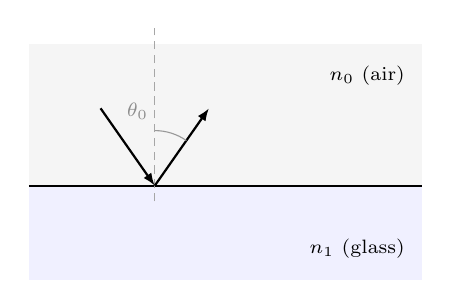
\begin{tikzpicture}
  \fill[black!4] (0,0) rectangle (5,1.8);
  \fill[blue!6]  (0,-1.2) rectangle (5,0);
  \draw[thick] (0,0) -- (5,0);
  \node[lbl, anchor=east] at (4.9, 1.4) {$n_0$ (air)};
  \node[lbl, anchor=east] at (4.9,-0.8) {$n_1$ (glass)};
  \raysketch{1.6}{35}{f}
\end{tikzpicture}
\end{center}

\begin{figure}[!htbp]
  \centering
  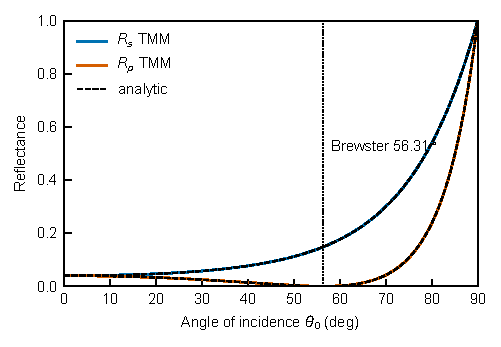
\includegraphics[width=0.5\textwidth]{01_fresnel_single_interface.pdf}
  \caption{Reflectance of an air/glass interface at \SI{550}{\nano\metre} for $s$- and $p$-polarisation. TMM (colour) coincides with the closed-form Fresnel result (dashed) at machine precision. The Brewster angle is marked by the dotted vertical line.}
  \label{fig:fresnel-single}
\end{figure}

The TMM reproduces the closed-form reflectance to
$\max|\Delta R| \approx \num{4e-13}$ across the full sweep, and
$|r_p(\theta_B)| \approx \num{3e-16}$ exactly at the Brewster angle. Both
residuals are at the level of double-precision floating-point noise, which
confirms that the single-interface coefficients are evaluated correctly
before any multilayer machinery is invoked.



\section{Fresnel with complex index}

The second example extends the single-interface benchmark to a complex
refractive index and adds the phase of the reflected amplitude as an
independent check. Two cases are evaluated side by side at
$\lambda = \SI{550}{\nano\metre}$: air ($n_0 = 1.00$) against a
non-absorbing glass substrate ($n_1 = 1.50$), and air against an absorbing
Si-like substrate ($n_1 = 4.00 + 0.05\,\ii$). The angle of incidence is
sampled from $0$ to \SI{89.5}{\degree} in 361 points. Because the substrate
can be complex, Snell's law and the cosine that enters
\eqref{eq:fresnel-rs}--\eqref{eq:fresnel-rp} must be evaluated on the
physical branch,
\begin{equation}
  \cos\theta_1 = \sqrt{1 - (n_0/n_1)^{2}\sin^{2}\theta_0},\qquad \Imy(\cos\theta_1)\ge 0, \label{eq:cos-branch}
\end{equation}
so that the transmitted wave decays into the absorbing half-space. At
normal incidence the two polarisations become physically indistinguishable
and the code returns
\begin{equation}
  r_s(0) = r_p(0) = \frac{n_0 - n_1}{n_0 + n_1}, \label{eq:fresnel2-normal}
\end{equation}
whereas the textbook formulas written in the opposite sign convention give
$r_s(0) = -r_p(0)$; the sign flip is applied once when overlaying the
analytic reference on the TMM curve.

\begin{center}
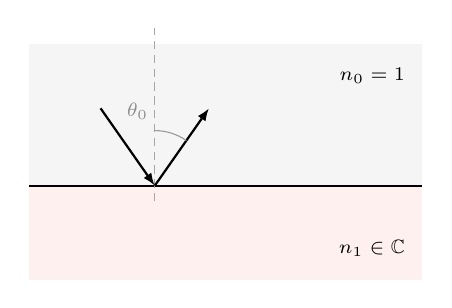
\begin{tikzpicture}
  \fill[black!4] (0,0) rectangle (5,1.8);
  \fill[red!6]   (0,-1.2) rectangle (5,0);
  \draw[thick] (0,0) -- (5,0);
  \node[lbl, anchor=east] at (4.9, 1.4) {$n_0=1$};
  \node[lbl, anchor=east] at (4.9,-0.8) {$n_1 \in \mathbb{C}$};
  \raysketch{1.6}{35}{f}
\end{tikzpicture}
\end{center}

\begin{figure}[!htbp]
  \centering
  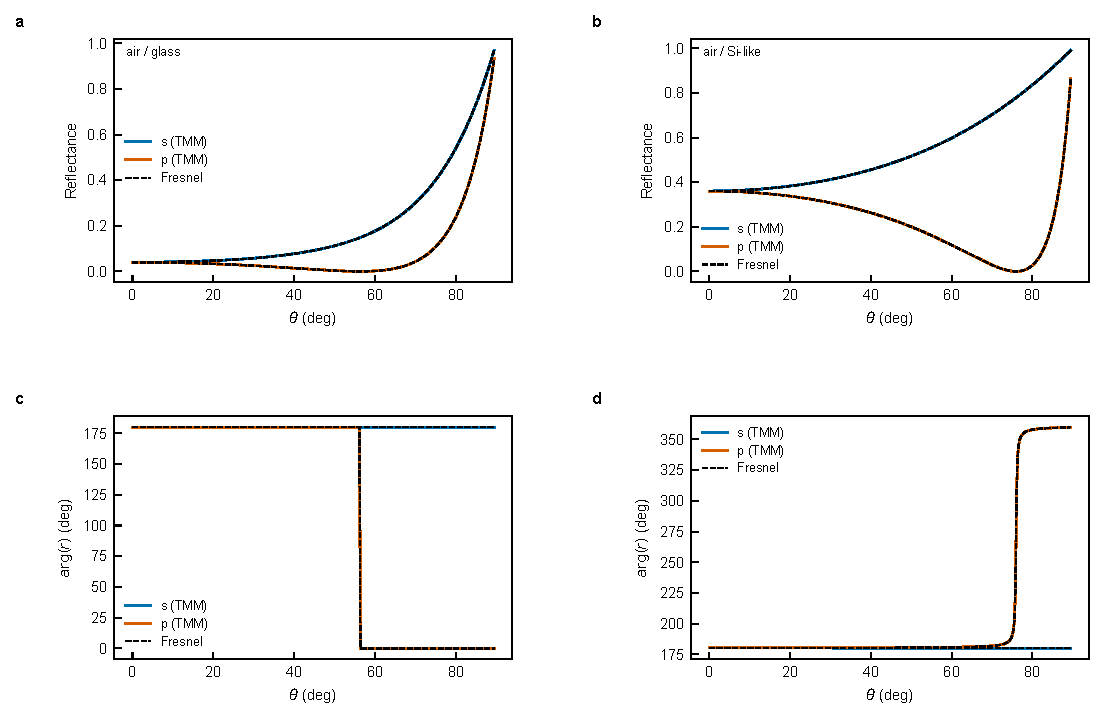
\includegraphics[width=\textwidth]{02_fresnel_analytic_check.pdf}
  \caption{TMM versus closed-form Fresnel for a real (glass) and a complex (Si-like) substrate. Panels (a,b) show $R_s(\theta)$ and $R_p(\theta)$; panels (c,d) show $\arg r_s$ and $\arg r_p$ over the same angular range.}
  \label{fig:fresnel2}
\end{figure}

With the sign convention fixed, amplitudes and phases coincide in all
four panels at $\max|\Delta R| \approx \num{6e-14}$. The dielectric case
shows the expected sharp Brewster zero and $\pi$ phase jump in $r_p$, while
the absorbing substrate replaces both by the smooth phase walk of
Fig.~\ref{fig:fresnel2}(d). The agreement across real and complex
substrates validates the branch-cut choice of~\eqref{eq:cos-branch}, which
is the single numerical subtlety that separates the complex case from the
real one.



\section{Total internal reflection and frustrated TIR}

The third example probes the same single-interface machinery beyond the
critical angle and then promotes the geometry to a three-layer stack in
order to resolve the evanescent tunnelling known as frustrated total
internal reflection (FTIR). The incident medium is glass ($n_1 = 1.50$)
and the transmitted medium is air ($n_2 = 1.00$) at
$\lambda = \SI{550}{\nano\metre}$, so the critical angle is
$\theta_c = \arcsin(n_2/n_1) = \SI{41.81}{\degree}$. Above $\theta_c$ no
real transmission angle exists; the normal component of the wavevector in
air becomes imaginary, and unitarity demands
\begin{equation}
  R(\theta > \theta_c) = 1. \label{eq:tir-R}
\end{equation}
Panel (a) of Fig.~\ref{fig:tir} plots $|1 - R|$ for $s$- and
$p$-polarisation on a logarithmic scale across the forbidden window
$\theta_c < \theta < \SI{89}{\degree}$. Panel (b) compares the unwrapped
phase of $r_s$ to the textbook closed form
\begin{equation}
  \tan\!\left(\frac{\delta_s}{2}\right) = \frac{\sqrt{\sin^{2}\theta - (n_2/n_1)^{2}}}{\cos\theta}. \label{eq:tir-phase}
\end{equation}

Panel (c) inserts a finite air gap of variable thickness $d$ between two
glass half-spaces, so the stack becomes glass\,/\,air\,/\,glass with a
single finite layer. Above $\theta_c$ the wave in the gap is evanescent,
with imaginary out-of-plane wavenumber $q_2 = \ii\kappa$ and
$\kappa = k_0\sqrt{n_1^{2}\sin^{2}\theta - n_2^{2}}$. The three-layer
Airy transmittance then reads
\begin{equation}
  t = \frac{t_{12}\,t_{21}\,e^{\ii q_2 d}}{1 - r_{12}^{2}\,e^{2\ii q_2 d}},\qquad T = |t|^{2}, \label{eq:ftir-T}
\end{equation}
which is evaluated at $\theta = \SI{60}{\degree}$ for gap thicknesses from
\SI{10}{\nano\metre} to \SI{600}{\nano\metre} and overlaid on the TMM
result.

\begin{center}
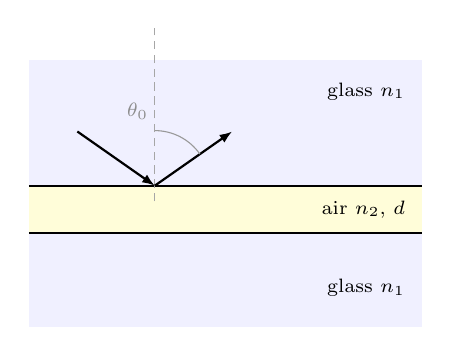
\begin{tikzpicture}
  \fill[blue!6]  (0, 0) rectangle (5, 1.6);
  \fill[yellow!15] (0,-0.6) rectangle (5, 0);
  \fill[blue!6]  (0,-1.8) rectangle (5,-0.6);
  \draw[thick] (0,0) -- (5,0);
  \draw[thick] (0,-0.6) -- (5,-0.6);
  \node[lbl, anchor=east] at (4.9, 1.2) {glass $n_1$};
  \node[lbl, anchor=east] at (4.9,-0.3) {air $n_2$, $d$};
  \node[lbl, anchor=east] at (4.9,-1.3) {glass $n_1$};
  \raysketch{1.6}{55}{t}
\end{tikzpicture}
\end{center}

\begin{figure}[!htbp]
  \centering
  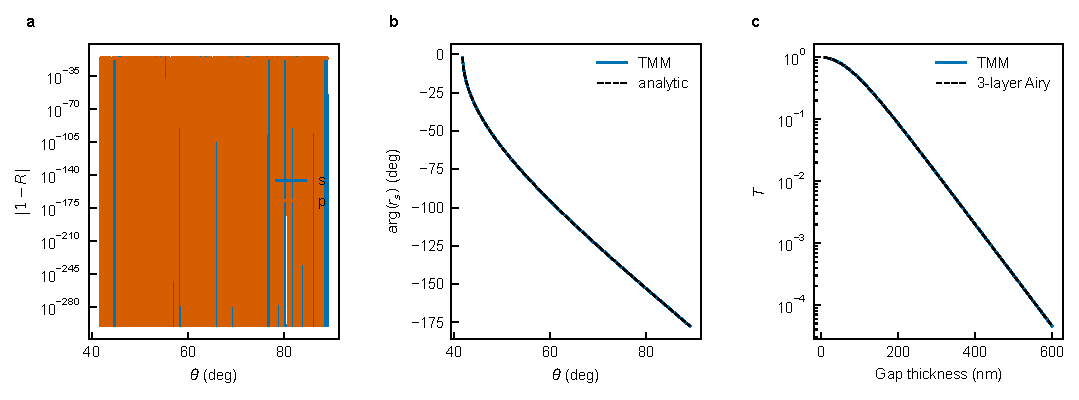
\includegraphics[width=\textwidth]{03_tir_and_ftir.pdf}
  \caption{(a) $|1-R|$ above $\theta_c$ for $s$ and $p$ polarisation. (b) Phase of $r_s$ versus the closed form~\eqref{eq:tir-phase}. (c) Frustrated-TIR transmittance $T(d)$ at \SI{60}{\degree} against the exact three-layer Airy expression~\eqref{eq:ftir-T}.}
  \label{fig:tir}
\end{figure}

Above $\theta_c$ the TMM returns unit reflectance to
$|1-R| \approx \num{9e-16}$ for both polarisations, and the reflection
phase tracks~\eqref{eq:tir-phase} to the same tolerance. The FTIR curve
agrees with the closed-form Airy transmittance at
$\max|\Delta T| \approx \num{7e-16}$ down to sub-nanometre gaps. The
transmittance follows the pure exponential $e^{-2\kappa d}$ for
$d \gg \kappa^{-1}$, but deviates visibly from it below
$d \lesssim \SI{100}{\nano\metre}$; in that near-gap regime the Fresnel
prefactors of~\eqref{eq:ftir-T} matter, and the TMM tracks those
corrections exactly.



\section{Thin-film Airy formula}

The fourth example pushes the benchmark from two to three media by placing
a single finite film between two half-spaces and comparing the TMM against
the closed-form Airy formula at normal incidence. Three configurations are
run in parallel, sweeping the wavelength from \SI{300}{\nano\metre} to
\SI{1000}{\nano\metre}:

\begin{itemize}
  \setlength{\itemsep}{0.2em}
  \item Case (a): air ($n_0 = 1$) / lossless film ($n_1 = 2.0$) / glass ($n_2 = 1.5$), film thickness $d = \SI{100}{\nano\metre}$;
  \item Case (b): air / absorbing film ($n_1 = 3.0 + 0.05\,\ii$) / glass, $d = \SI{500}{\nano\metre}$;
  \item Case (c): air / absorbing film ($n_1 = 3.0 + 0.05\,\ii$) / absorbing substrate ($n_2 = 3.11 + 4.89\,\ii$), $d = \SI{500}{\nano\metre}$.
\end{itemize}

Case (a) is purely interferometric, case (b) adds weak absorption in the
film, and case (c) makes both the film and the substrate complex, which
tests the branch-cut convention of both the film wavenumber and the
substrate Fresnel coefficient simultaneously. The analytic reference is
the Airy formula for a single film,
\begin{equation}
  r = \frac{r_{01} + r_{12}\,e^{2\ii\beta}}{1 + r_{01}\,r_{12}\,e^{2\ii\beta}},\qquad \beta = \frac{2\pi n_1 d}{\lambda}\cos\theta_1, \label{eq:airy-r}
\end{equation}
with $r_{jk}$ the single-interface amplitudes
of~\eqref{eq:fresnel-rs}--\eqref{eq:fresnel-rp}. The positive sign in
$e^{+2\ii\beta}$ is dictated by the $e^{-\ii\omega t}$ time convention and
is the sign that makes~\eqref{eq:airy-r} consistent with the Fresnel
amplitudes used by the TMM.

\begin{center}
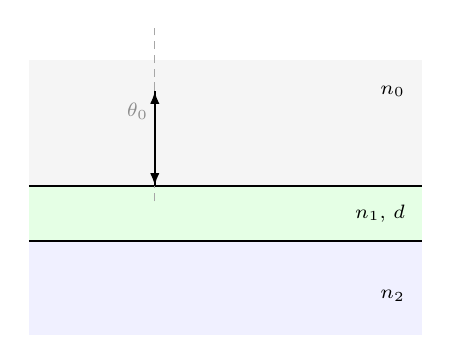
\begin{tikzpicture}
  \fill[black!4] (0, 0) rectangle (5, 1.6);
  \fill[green!10] (0,-0.7) rectangle (5, 0);
  \fill[blue!6]  (0,-1.9) rectangle (5,-0.7);
  \draw[thick] (0,0) -- (5,0);
  \draw[thick] (0,-0.7) -- (5,-0.7);
  \node[lbl, anchor=east] at (4.9, 1.2) {$n_0$};
  \node[lbl, anchor=east] at (4.9,-0.35) {$n_1$, $d$};
  \node[lbl, anchor=east] at (4.9,-1.4) {$n_2$};
  \raysketch{1.6}{0}{f}
\end{tikzpicture}
\end{center}

\begin{figure}[!htbp]
  \centering
  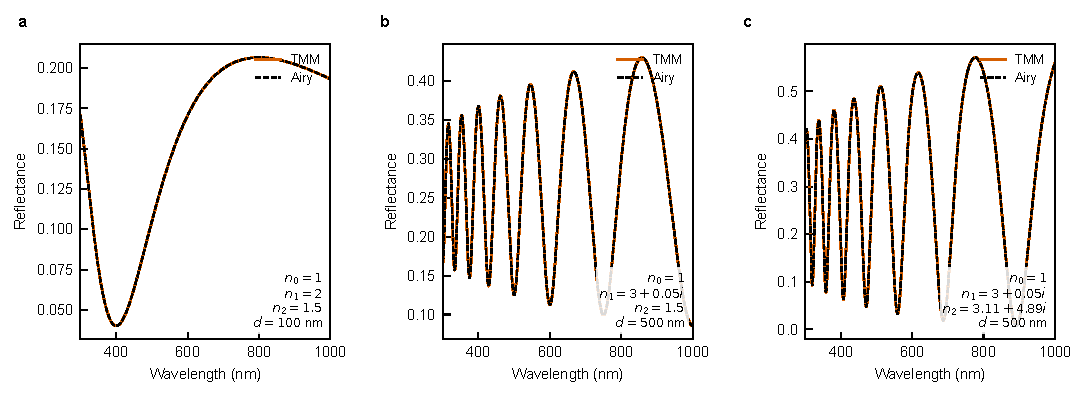
\includegraphics[width=\textwidth]{04_thin_film_airy.pdf}
  \caption{Reflectance of a single film versus wavelength for the three cases listed in the text. TMM (solid colour) overlays the Airy formula (dashed black) in each panel.}
  \label{fig:airy}
\end{figure}

Across all three cases the TMM and Airy curves coincide at
$\max|R_{\rm TMM} - R_{\rm Airy}| \approx \num{4e-15}$, independent of
whether the film or the substrate is absorbing. The residual is dominated
by the catastrophic cancellation that enters~\eqref{eq:airy-r} when the
numerator is nearly zero, and it stays at the level of floating-point
noise throughout the scan. Case (a) shows the textbook equally-spaced Airy
fringes, case (b) damps the fringe contrast towards shorter wavelengths as
the film absorption becomes significant, and case (c) adds a smooth
background from the complex substrate Fresnel coefficient on which the
attenuated fringes ride.



\section{Half-wave and quarter-wave identities}

Two classical design identities of single-layer interferometry are checked
at the design wavelength $\lambda_0 = \SI{550}{\nano\metre}$. Both use a
three-layer stack (incident medium, film, substrate) at normal incidence
and are scanned across \SIrange{400}{800}{\nano\metre} for context.

The first panel realises the half-wave \emph{invisible} layer: a lossless
film of index $n_f = 2.0$ is placed on glass ($n_s = 1.5$) in air
($n_0 = 1.0$), with thickness
\begin{equation}
  d_{\rm HW} = \frac{\lambda_0}{2 n_f} = \SI{137.5}{\nano\metre}. \label{eq:hw-d}
\end{equation}
At $\lambda_0$ the film introduces a round-trip phase of $2\pi$, so the
internal Airy factor in~\eqref{eq:airy-r} reduces to unity and the
reflectance of the stack at that wavelength collapses to the bare-substrate
value,
\begin{equation}
  R(\lambda_0) = \left(\frac{n_0 - n_s}{n_0 + n_s}\right)^{2}. \label{eq:hw-R}
\end{equation}

The second panel realises the index-matched quarter-wave antireflection
(AR) film: the film index is chosen as the geometric mean
$n_f = \sqrt{n_0 n_s} \approx 1.225$, the thickness is
\begin{equation}
  d_{\rm QW} = \frac{\lambda_0}{4 n_f}, \label{eq:qw-d}
\end{equation}
and~\eqref{eq:airy-r} then gives exact destructive interference at
$\lambda_0$,
\begin{equation}
  R(\lambda_0) = 0. \label{eq:qw-R}
\end{equation}

\begin{center}
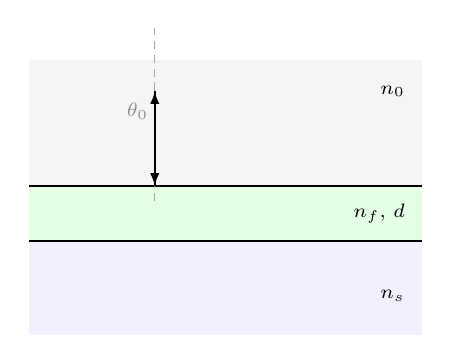
\begin{tikzpicture}
  \fill[black!4] (0, 0) rectangle (5, 1.6);
  \fill[green!10] (0,-0.7) rectangle (5, 0);
  \fill[blue!6]  (0,-1.9) rectangle (5,-0.7);
  \draw[thick] (0,0) -- (5,0);
  \draw[thick] (0,-0.7) -- (5,-0.7);
  \node[lbl, anchor=east] at (4.9, 1.2) {$n_0$};
  \node[lbl, anchor=east] at (4.9,-0.35) {$n_f$, $d$};
  \node[lbl, anchor=east] at (4.9,-1.4) {$n_s$};
  \raysketch{1.6}{0}{f}
\end{tikzpicture}
\end{center}

\begin{figure}[!htbp]
  \centering
  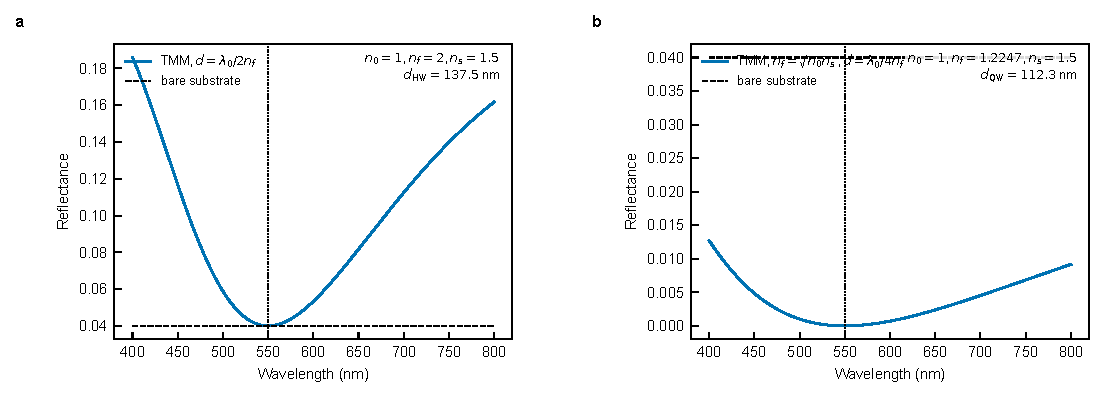
\includegraphics[width=\textwidth]{05_halfwave_quarterwave.pdf}
  \caption{(a) Half-wave invisible film returns the bare-substrate reflectance at $\lambda_0$. (b) Index-matched quarter-wave antireflection film gives zero reflectance at $\lambda_0$ and a smooth V-shape across the scan.}
  \label{fig:hwqw}
\end{figure}

At $\lambda_0$ the half-wave film coincides with the bare substrate to
$|R_{\rm film}(\lambda_0) - R_{\rm bare}| \approx \num{3e-17}$, and the
index-matched quarter-wave film reaches $R(\lambda_0) \approx \num{6e-33}$;
the latter is a squared amplitude and therefore registers the reflection
amplitude itself vanishing at the level of $\sqrt{\num{6e-33}} \sim
\num{8e-17}$, i.e.\ pure floating-point zero. The two identities
constrain the Airy phase and the Fresnel zero condition independently, so
their simultaneous satisfaction is a stronger check than either one alone.



\section{Single-layer antireflection coating}

Beyond the idealised index-matched case of the previous section, the
quarter-wave AR formula predicts a finite residual reflectance whenever
the film index is not exactly $\sqrt{n_0 n_s}$. The benchmark here is a
magnesium-fluoride film ($n_f = 1.38$) on crown glass ($n_s = 1.52$) in
air ($n_0 = 1.00$) at the design wavelength
$\lambda_0 = \SI{550}{\nano\metre}$. The analytical optimum thickness and
residual reflectance are
\begin{align}
  d_{\rm opt} &= \frac{\lambda_0}{4 n_f} \approx \SI{99.6}{\nano\metre}, \label{eq:ar-d}\\[2pt]
  R_{\min}    &= \left(\frac{n_0 n_s - n_f^{2}}{n_0 n_s + n_f^{2}}\right)^{2}. \label{eq:ar-Rmin}
\end{align}
$R_{\min}$ is the exact reflectance of the stack at $\lambda_0$ when
$d = d_{\rm opt}$; it vanishes only in the index-matched limit
$n_f^{2} = n_0 n_s$.

Two independent scans are performed: panel (a) fixes the wavelength at
$\lambda_0$ and sweeps the film thickness from $0$ to \SI{300}{\nano\metre}
on a 601-point grid, locating the analytic minimum; panel (b) fixes the
thickness at $d_{\rm opt}$ and sweeps the wavelength across
\SIrange{400}{700}{\nano\metre}, overlaying the bare-substrate reflectance
for reference.

\begin{center}
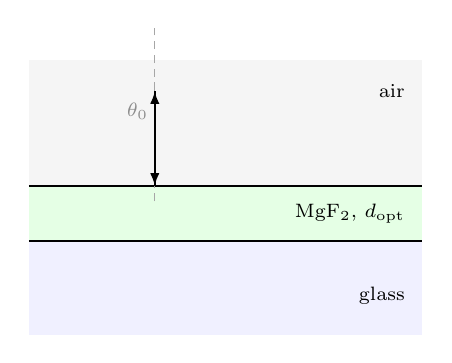
\begin{tikzpicture}
  \fill[black!4] (0, 0) rectangle (5, 1.6);
  \fill[green!10] (0,-0.7) rectangle (5, 0);
  \fill[blue!6]  (0,-1.9) rectangle (5,-0.7);
  \draw[thick] (0,0) -- (5,0);
  \draw[thick] (0,-0.7) -- (5,-0.7);
  \node[lbl, anchor=east] at (4.9, 1.2) {air};
  \node[lbl, anchor=east] at (4.9,-0.35) {MgF$_2$, $d_{\rm opt}$};
  \node[lbl, anchor=east] at (4.9,-1.4) {glass};
  \raysketch{1.6}{0}{f}
\end{tikzpicture}
\end{center}

\begin{figure}[!htbp]
  \centering
  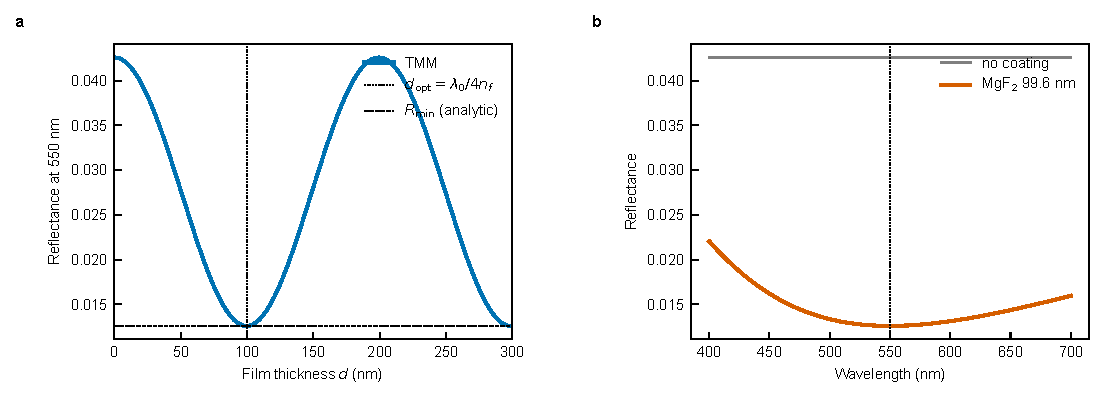
\includegraphics[width=\textwidth]{06_antireflection_coating.pdf}
  \caption{(a) Reflectance as a function of film thickness at $\lambda_0 = \SI{550}{\nano\metre}$, touching the analytic $R_{\min}$ at $d = d_{\rm opt}$. (b) Reflectance against wavelength at the optimum thickness, with the bare-substrate curve overlaid for comparison.}
  \label{fig:ar}
\end{figure}

The minimum of the TMM thickness scan falls exactly
on~\eqref{eq:ar-Rmin} with
$|R_{\rm TMM}(d_{\rm opt}, \lambda_0) - R_{\min}| \approx \num{7e-18}$, and
the wavelength scan shows the familiar broadband V-shape touching the
analytic $R_{\min}$ only at the design wavelength. The residual
reflectance (here $R_{\min} \approx \num{1.3e-2}$) is a pure consequence of
the index mismatch between MgF$_2$ and the glass--air geometry; broadening
the AR spectrally requires multilayer designs, which are addressed by the
Bragg and bandpass examples below.



\section{Absorbing layer: energy conservation and Beer--Lambert limit}

With absorption present in a finite layer, the reflectance and the
transmittance no longer sum to unity; the missing fraction is deposited in
the film itself. This example verifies, first, that the TMM partitions the
incident power correctly ($R + T + A = 1$) and, second, that the
transmittance approaches the expected Beer--Lambert exponential for
optically thick films. The stack is an amorphous-silicon-like film
($n_f = 4.0 + 0.5\,\ii$) on glass ($n_s = 1.52$) in air ($n_0 = 1.00$) at
$\lambda = \SI{550}{\nano\metre}$.

Panel (a) sweeps the film thickness from $0$ to \SI{400}{\nano\metre} in
801 points. The TMM returns the reflectance $R$, the transmittance $T$ and
the per-layer absorption $A$ (here a single scalar because there is only
one finite layer). The three components oscillate through Airy fringes as
$d$ grows, but energy conservation
\begin{equation}
  R + T + A = 1 \label{eq:abs-rta}
\end{equation}
must hold at every point. Panel (b) extends the scan out to
\SI{2000}{\nano\metre}, where the Airy ripple in $T(d)$ decays into the
Beer--Lambert asymptote
\begin{equation}
  T(d) \longrightarrow T_{\rm if}\,e^{-\alpha d},\qquad \alpha = \frac{4\pi\,\Imy(n_f)}{\lambda}, \label{eq:abs-BL}
\end{equation}
with the interface transmittance
$T_{\rm if} = (1 - R_{\rm front})(1 - R_{\rm back})$ built from the two
single-interface reflectances. At $\lambda = \SI{550}{\nano\metre}$ the
numerical values are $\alpha \approx \SI{1.14e-2}{\per\nano\metre}$, i.e.\
a penetration depth $1/\alpha \approx \SI{87.5}{\nano\metre}$.

\begin{center}
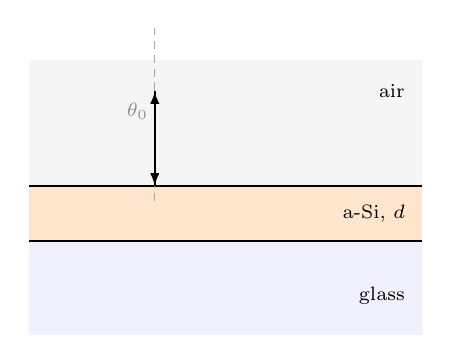
\begin{tikzpicture}
  \fill[black!4] (0, 0) rectangle (5, 1.6);
  \fill[orange!20] (0,-0.7) rectangle (5, 0);
  \fill[blue!6]  (0,-1.9) rectangle (5,-0.7);
  \draw[thick] (0,0) -- (5,0);
  \draw[thick] (0,-0.7) -- (5,-0.7);
  \node[lbl, anchor=east] at (4.9, 1.2) {air};
  \node[lbl, anchor=east] at (4.9,-0.35) {a-Si, $d$};
  \node[lbl, anchor=east] at (4.9,-1.4) {glass};
  \raysketch{1.6}{0}{t}
\end{tikzpicture}
\end{center}

\begin{figure}[!htbp]
  \centering
  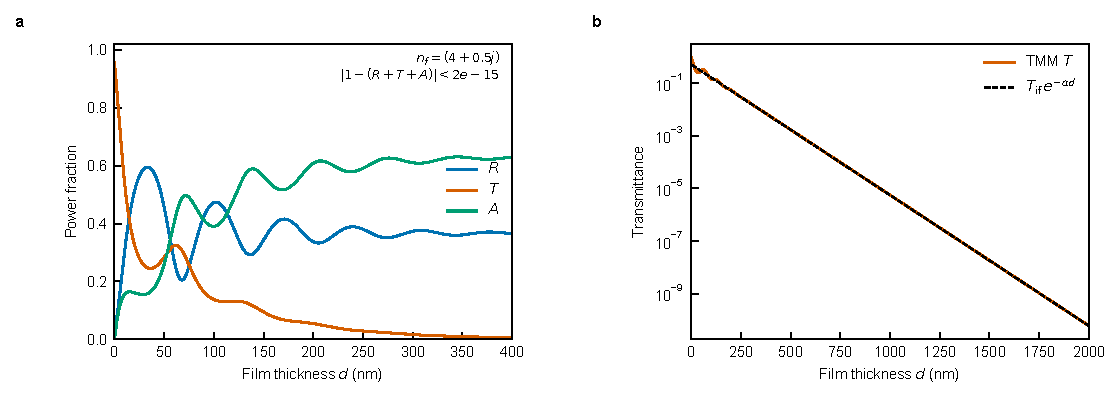
\includegraphics[width=\textwidth]{07_absorbing_layer.pdf}
  \caption{(a) Reflectance $R$, transmittance $T$ and per-layer absorption $A$ as a function of film thickness. (b) $T(d)$ on a logarithmic scale out to \SI{2000}{\nano\metre}, with the Beer--Lambert envelope $T_{\rm if}\,e^{-\alpha d}$ as a reference.}
  \label{fig:absorb}
\end{figure}

Equation~\eqref{eq:abs-rta} is satisfied to
$\max|1 - (R + T + A)| \approx \num{2e-15}$ over the whole thickness
scan, which confirms the per-layer absorption formula derived from the
Poynting flux balance. For $d \gtrsim 1/\alpha$ the oscillatory Fabry--Pérot
modulation of $T(d)$ dies out, and beyond a few absorption lengths the TMM
curve locks onto the exponential envelope of~\eqref{eq:abs-BL} without
adjustable parameters. The transition from coherent interference to the
Beer--Lambert regime is therefore reproduced smoothly by the same
formalism.



\section{Beer--Lambert depth profile in a metal}

The per-layer absorption returned by the TMM can be used to resolve the
spatial deposition of optical power with arbitrary resolution. This
benchmark slices a gold half-space into $N = 100$ virtual layers of
$dz = \SI{2}{\nano\metre}$ each, followed by a bulk gold half-space as
substrate, so the total thickness (\SI{200}{\nano\metre}) is deep enough
that the reflectance has converged to the bulk Fresnel value. The gold
refractive index at $\lambda = \SI{550}{\nano\metre}$ is taken from the
Johnson--Christy tabulation as $n_{\rm Au} = 0.425 + 2.367\,\ii$. Because
all $N$ slices carry the same index as the substrate, the slicing is a
pure reparametrisation of a continuous absorber.

With the field entering the metal at intensity $I_{\rm in} = 1 - R$ and
the absorption coefficient
$\alpha = 4\pi\,\Imy(n_{\rm Au})/\lambda$, the differential and
cumulative Beer--Lambert expressions are
\begin{align}
  \frac{\mathrm{d}A}{\mathrm{d}z} &= \alpha\,I_{\rm in}\,e^{-\alpha z}, \label{eq:bl-diff}\\[2pt]
  A(<z) &= I_{\rm in}\bigl(1 - e^{-\alpha z}\bigr). \label{eq:bl-cum}
\end{align}
Panel (a) compares the TMM per-layer absorption $A_j$, evaluated at the
midpoint depth $z_j = (j - 1/2)\,dz$, against
$\alpha\,dz\,(1 - R)\,e^{-\alpha z_j}$. Panel (b) overlays the cumulative
sum $\sum_{k \le j} A_k$ on the closed form~\eqref{eq:bl-cum}.

\begin{center}
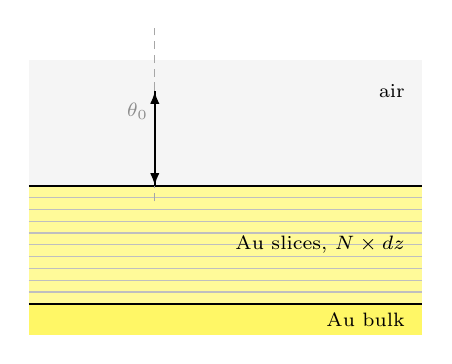
\begin{tikzpicture}
  \fill[black!4] (0, 0) rectangle (5, 1.6);
  \foreach \i in {0,...,9} {
    \fill[yellow!40] (0,{-0.15*(\i+1)}) rectangle (5, {-0.15*\i});
    \draw[thin, gray!50] (0,{-0.15*\i}) -- (5,{-0.15*\i});
  }
  \fill[yellow!60] (0,-1.9) rectangle (5,-1.5);
  \draw[thick] (0,0) -- (5,0);
  \draw[thick] (0,-1.5) -- (5,-1.5);
  \node[lbl, anchor=east] at (4.9, 1.2) {air};
  \node[lbl, anchor=east] at (4.9,-0.75) {Au slices, $N \times dz$};
  \node[lbl, anchor=east] at (4.9,-1.7) {Au bulk};
  \raysketch{1.6}{0}{f}
\end{tikzpicture}
\end{center}

\begin{figure}[!htbp]
  \centering
  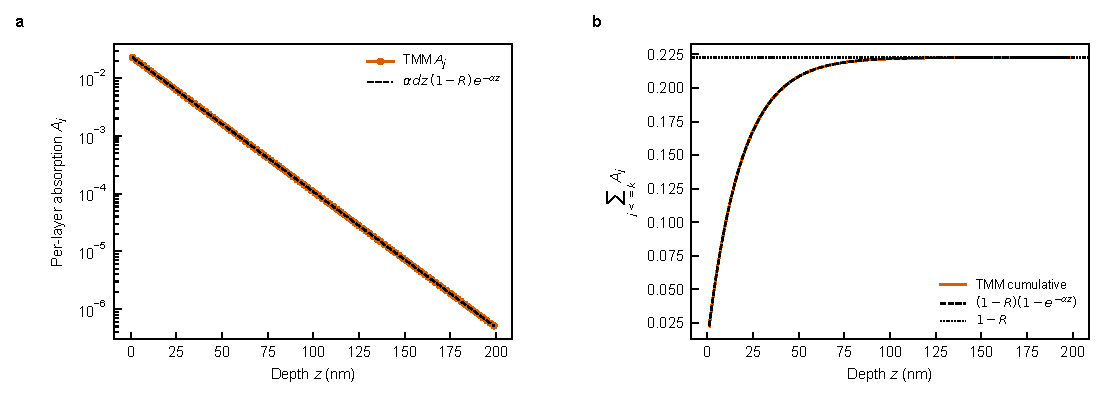
\includegraphics[width=\textwidth]{08_beer_lambert.pdf}
  \caption{(a) Per-layer absorption $A_j$ at slice midpoints, TMM versus the Beer--Lambert prediction. (b) Cumulative absorption up to depth $z$, TMM against the closed form~\eqref{eq:bl-cum}.}
  \label{fig:beer}
\end{figure}

The cumulative curve matches~\eqref{eq:bl-cum} to
$\max|A_{\rm cum,TMM} - A_{\rm cum,BL}| \approx \num{1e-15}$, which
confirms the total energy partition of the TMM. The differential
form~\eqref{eq:bl-diff} shows a residual of order $\num{5e-4}$ near the
surface; this is not a methodological bias but the finite-difference error
$\mathcal{O}(\alpha^{2}\,dz^{2})$ inherent to approximating
$\int_{z_j - dz/2}^{z_j + dz/2} e^{-\alpha z}\,\mathrm{d}z$ by the midpoint
value times $dz$. Halving the slice thickness to \SI{1}{\nano\metre}
reduces the residual to $\sim \num{1e-4}$, consistent with the quadratic
scaling.



\section{Metal reflectance of silver and gold}

This example uses experimental optical constants instead of fabricated
values. The refractive index of silver and gold is taken from the
Johnson--Christy tabulation sampled
at the ten wavelengths \SI{400}{}, \SI{450}{}, \SI{500}{}, \SI{550}{},
\SI{600}{}, \SI{650}{}, \SI{700}{}, \SI{800}{}, \SI{900}{},
\SI{1000}{\nano\metre}, and linearly interpolated on a 601-point grid
between $\SI{400}{}$ and $\SI{1000}{\nano\metre}$. The stack is reduced to
two half-spaces, air against metal, and the reflectance is evaluated at
normal incidence for both materials.

For a bare interface the $s$- and $p$-polarisations coincide, and the
normal-incidence reflectance follows directly from the Fresnel
coefficients as
\begin{equation}
  R = \frac{(n - 1)^{2} + k^{2}}{(n + 1)^{2} + k^{2}}, \label{eq:metal-R}
\end{equation}
with $N = n + \ii k$ the complex refractive index at the given wavelength.
Equation~\eqref{eq:metal-R} is the strong reference against which the TMM
result is compared: any disagreement would indicate an error in the
branch-cut choice for complex $N$ or in the evaluation of the
single-interface Fresnel coefficient at $\theta_0 = 0$.

\begin{center}
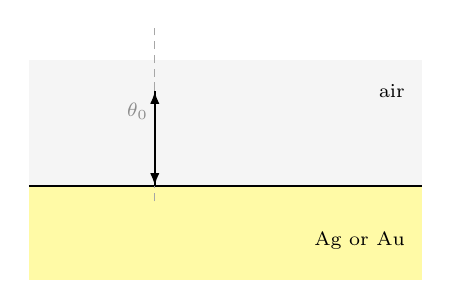
\begin{tikzpicture}
  \fill[black!4]   (0, 0) rectangle (5, 1.6);
  \fill[yellow!35] (0,-1.2) rectangle (5, 0);
  \draw[thick] (0,0) -- (5,0);
  \node[lbl, anchor=east] at (4.9, 1.2) {air};
  \node[lbl, anchor=east] at (4.9,-0.7) {Ag or Au};
  \raysketch{1.6}{0}{f}
\end{tikzpicture}
\end{center}

\begin{figure}[!htbp]
  \centering
  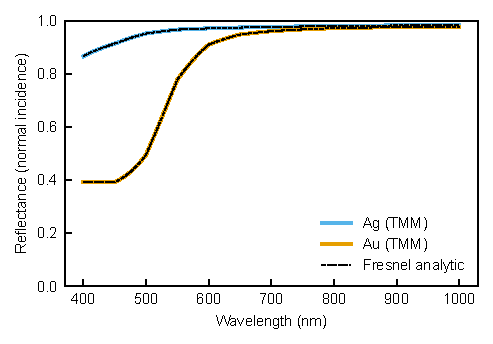
\includegraphics[width=0.5\textwidth]{09_metal_reflectance.pdf}
  \caption{Reflectance of bulk silver and bulk gold from \SIrange{400}{1000}{\nano\metre} at normal incidence. TMM (solid) is overlaid on the closed-form Fresnel expression~\eqref{eq:metal-R} evaluated from the same tabulated $N(\lambda)$.}
  \label{fig:metal}
\end{figure}

The TMM reproduces~\eqref{eq:metal-R} at
$\max|\Delta R| \approx \num{1e-15}$ for silver and $\num{9e-16}$ for
gold. Silver remains above $R \approx 0.95$ across the whole visible and
near-infrared range; gold shows the characteristic absorption edge that
pulls the reflectance down below \SI{500}{\nano\metre}, with the
reflectance rising again and saturating near unity in the red and
near-infrared. The identity of the two curves to floating-point precision
confirms that tabulated complex indices are ingested and propagated
consistently by the code.



\section{Distributed Bragg reflector}

The first genuine multilayer benchmark is a quarter-wave distributed
Bragg reflector (DBR). The stack alternates a high-index and a low-index
quarter-wave layer and is repeated $N$ times on a glass substrate. The
materials are TiO$_2$ ($n_H = 2.35$) and SiO$_2$ ($n_L = 1.38$) on glass
($n_s = 1.52$) in air ($n_0 = 1.00$), with the design wavelength fixed at
$\lambda_0 = \SI{550}{\nano\metre}$. Each layer thickness equals one
optical quarter-wavelength, so
$d_H = \lambda_0/(4 n_H) \approx \SI{58.5}{\nano\metre}$ and
$d_L = \lambda_0/(4 n_L) \approx \SI{99.6}{\nano\metre}$. The refractive
index list fed to the TMM is
\[
  (n_0,\ n_H,\ n_L,\ n_H,\ n_L,\ \ldots,\ n_H,\ n_L,\ n_s),
\]
with the $(n_H, n_L)$ block repeated $N$ times, and the thickness list is
the corresponding $(d_H, d_L)^{N}$ sequence.

Two analytical results frame the behaviour. The width of the high-reflectance
stopband centred at $\lambda_0$ is
\begin{equation}
  \frac{\Delta\lambda}{\lambda_0} = \frac{4}{\pi}\arcsin\!\left(\frac{n_H - n_L}{n_H + n_L}\right), \label{eq:dbr-band}
\end{equation}
and the peak reflectance at $\lambda_0$, with the effective substrate
admittance $Y_{\rm eff} = (n_H/n_L)^{2N}\,n_s$ for the stack terminated in
$n_L$\,/\,substrate, is
\begin{equation}
  R_{\rm peak} = \left(\frac{n_0 - Y_{\rm eff}}{n_0 + Y_{\rm eff}}\right)^{2}. \label{eq:dbr-Rpeak}
\end{equation}
Panel (a) plots $R(\lambda)$ across \SIrange{400}{800}{\nano\metre} for
$N = 2, 5, 10$ pairs with the stopband from~\eqref{eq:dbr-band} shaded.
Panel (b) sweeps $N$ from $1$ to $15$ and compares the TMM peak reflectance
at $\lambda_0$ with~\eqref{eq:dbr-Rpeak}.

\begin{center}
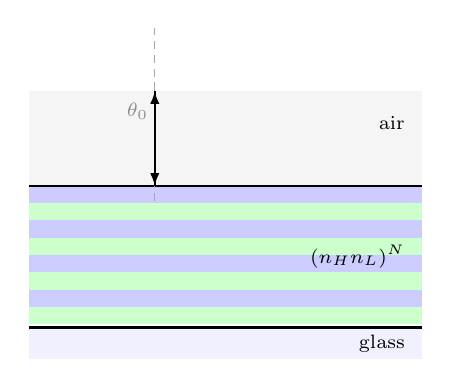
\begin{tikzpicture}
  \fill[black!4] (0, 0) rectangle (5, 1.2);
  \foreach \i in {0,...,3} {
    \fill[blue!20]  (0,{-0.22*(2*\i+1)}) rectangle (5, {-0.22*(2*\i)});
    \fill[green!20] (0,{-0.22*(2*\i+2)}) rectangle (5, {-0.22*(2*\i+1)});
  }
  \fill[blue!6] (0,-2.2) rectangle (5,-1.8);
  \draw[thick] (0,0) -- (5,0);
  \draw[thick] (0,-1.8) -- (5,-1.8);
  \node[lbl, anchor=east] at (4.9, 0.8) {air};
  \node[lbl, anchor=east] at (4.9,-0.9) {$(n_H n_L)^N$};
  \node[lbl, anchor=east] at (4.9,-2.0) {glass};
  \raysketch{1.6}{0}{f}
\end{tikzpicture}
\end{center}

\begin{figure}[!htbp]
  \centering
  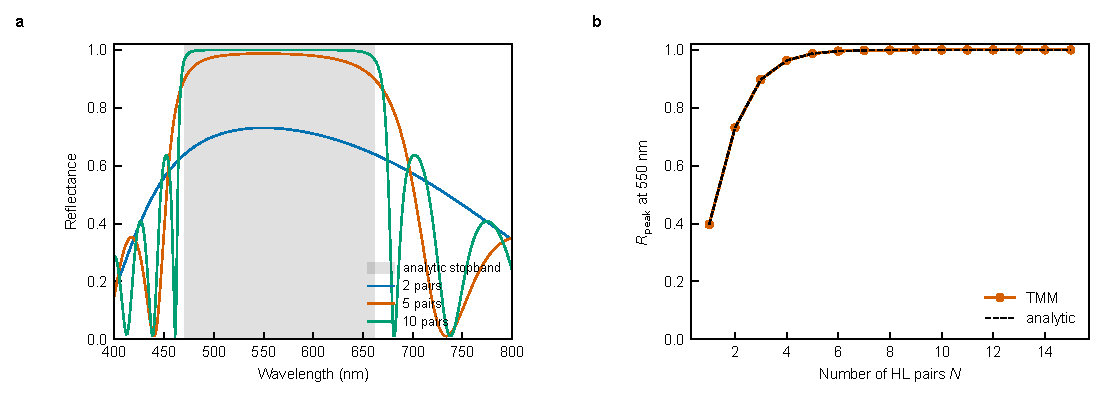
\includegraphics[width=\textwidth]{10_bragg_mirror.pdf}
  \caption{(a) Reflectance of the DBR for $N = 2, 5, 10$ pairs on glass; the shaded band marks the analytic stopband~\eqref{eq:dbr-band}. (b) Peak reflectance at $\lambda_0$ against the admittance formula~\eqref{eq:dbr-Rpeak}.}
  \label{fig:bragg}
\end{figure}

The TMM peak reflectance tracks the admittance formula~\eqref{eq:dbr-Rpeak}
over $N = 1\ldots 15$ with
$|\Delta R_{\rm peak}| \approx \num{1e-15}$, and the high-reflectance
window in panel (a) falls inside the analytic stopband at all pair counts.
For $N \gtrsim 10$ the reflectance saturates above $99.99\%$ at the design
wavelength, and the stopband edges become progressively sharper with
increasing $N$; outside the stopband the curves show the usual ripple from
the finite number of periods, which the TMM reproduces in amplitude and
phase.



\section{Angle--wavelength map of a bandpass filter}

This example generalises the DBR benchmark to a two-dimensional scan in
wavelength and angle of incidence, using the simplest optical layout that
exhibits a narrow transmission passband: a single half-wave cavity placed
between two identical quarter-wave mirrors. Explicitly, the refractive
index list fed to the TMM at design wavelength
$\lambda_0 = \SI{550}{\nano\metre}$ is
\[
  \underbrace{\text{air}}_{n_0=1.00}\
  \underbrace{(n_H\,n_L)^{4}}_{\text{mirror 1}}\
  \underbrace{n_H}_{\text{spacer}}\
  \underbrace{(n_L\,n_H)^{4}}_{\text{mirror 2}}\
  \underbrace{\text{glass}}_{n_s = 1.52},
\]
with $n_H = 2.35$ and $n_L = 1.38$. The seventeen finite layers carry the
thicknesses $(d_H, d_L)^{4}$ for the first mirror, $d_{\rm cav}$ for the
spacer, and $(d_L, d_H)^{4}$ for the second mirror, where
\begin{equation}
  d_H = \frac{\lambda_0}{4 n_H},\quad d_L = \frac{\lambda_0}{4 n_L},\quad d_{\rm cav} = \frac{\lambda_0}{2 n_H}. \label{eq:map-thick}
\end{equation}
The spacer is therefore a \emph{half}-wave high-index layer, which
introduces a sharp transmission resonance at $\lambda_0$ sitting inside
the mirror stopband. The high-reflectance blocks on either side of the
cavity give the filter its narrow-band character; the cavity phase alone
sets the position of the passband.

The map scans $\lambda$ from $\SI{500}{}$ to $\SI{600}{\nano\metre}$ on
201 points and the angle of incidence $\theta_0$ from $0$ to
\SI{40}{\degree} on 41 points, for both $s$- and $p$-polarisation. At
oblique incidence the resonance shifts to shorter wavelengths because the
round-trip phase in the cavity picks up a factor of $\cos\theta_{\rm cav}$;
a first-order estimate treats the cavity as a single effective medium with
index $n_{\rm eff} \simeq \sqrt{n_H n_L}$, giving the textbook passband
shift
\begin{equation}
  \lambda(\theta) = \lambda_0\sqrt{1 - \frac{\sin^{2}\theta_0}{n_{\rm eff}^{2}}}. \label{eq:map-shift}
\end{equation}
Equation~\eqref{eq:map-shift} is the standard approximation for thin-film
bandpass filters and is accurate to a few per mille for modest angular
excursions; it is plotted as a dashed red curve on top of both maps.

\begin{center}
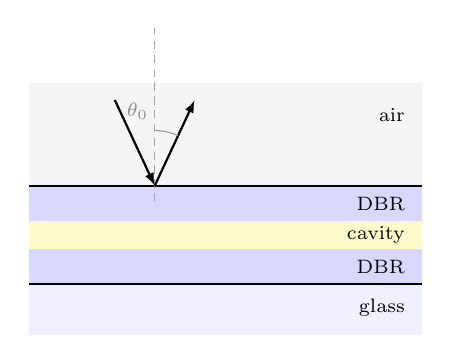
\begin{tikzpicture}
  \fill[black!4] (0, 0) rectangle (5, 1.3);
  \fill[blue!15] (0,-0.45) rectangle (5, 0);
  \fill[yellow!20] (0,-0.8) rectangle (5,-0.45);
  \fill[blue!15] (0,-1.25) rectangle (5,-0.8);
  \fill[blue!6]  (0,-1.9) rectangle (5,-1.25);
  \draw[thick] (0,0) -- (5,0);
  \draw[thick] (0,-1.25) -- (5,-1.25);
  \node[lbl, anchor=east] at (4.9, 0.9) {air};
  \node[lbl, anchor=east] at (4.9,-0.225){DBR};
  \node[lbl, anchor=east] at (4.9,-0.625){cavity};
  \node[lbl, anchor=east] at (4.9,-1.025){DBR};
  \node[lbl, anchor=east] at (4.9,-1.55){glass};
  \raysketch{1.6}{25}{f}
\end{tikzpicture}
\end{center}

\begin{figure}[!htbp]
  \centering
  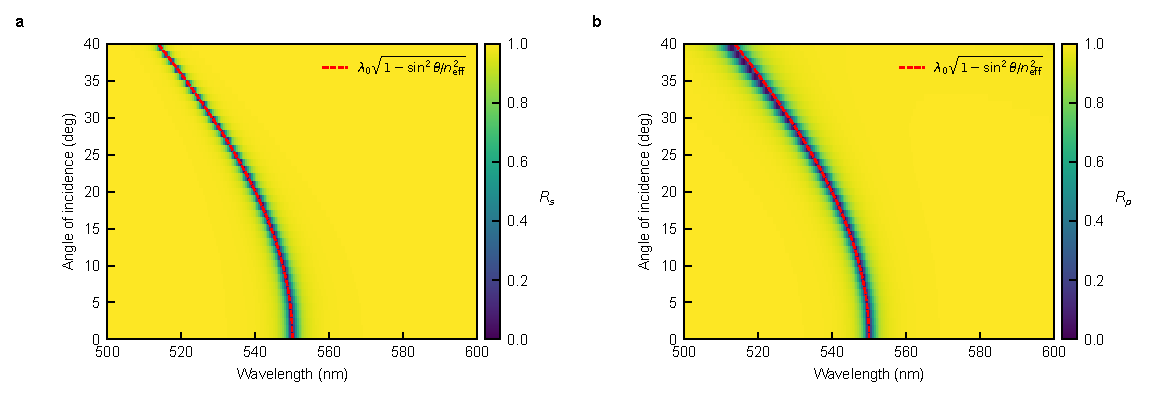
\includegraphics[width=\textwidth]{11_angle_wavelength_map.pdf}
  \caption{Two-dimensional reflectance map $R(\theta_0, \lambda)$ of the bandpass filter for $s$ (a) and $p$ (b) polarisation. The dark vertical streak is the narrow cavity resonance, seen here as a dip in reflectance; the dashed red curve is the analytic passband shift of equation~\eqref{eq:map-shift} with $n_{\rm eff} = \sqrt{n_H n_L}$.}
  \label{fig:map}
\end{figure}

The analytic curve tracks the minimum of $R(\theta_0, \lambda)$ in both
maps without adjustable parameters, which validates the angular dispersion
of the stack up to the approximation used in $n_{\rm eff}$. A second
feature emerges at oblique incidence: the $s$ and $p$ maps are no longer
identical. The $p$ map shows a shallower and slightly broader dip at large
$\theta_0$ because each interface carries a different Fresnel coefficient
for $p$ polarisation, which reduces the effective mirror reflectance and
broadens the cavity line. This polarisation splitting of the passband is
the exact quantity that tilted-incidence bandpass filters are designed
around, and it is reproduced here from first principles without any
effective-medium fit parameter.



\section{Fabry--P\'erot finesse versus mirror reflectance}

The previous example introduced the single-cavity bandpass geometry as a
sharp feature on top of a high-reflectance background. Here the same
building block is evaluated quantitatively: the transmittance spectrum of
a symmetric Fabry--P\'erot etalon is simulated for a range of mirror
reflectances, and the finesse extracted from the TMM is compared to the
analytic Airy prediction. The design wavelength is
$\lambda_0 = \SI{1000}{\nano\metre}$.

The etalon is built from two identical quarter-wave mirrors surrounding a
long air cavity. With $n_H = 2.35$, $n_L = 1.46$ (SiO$_2$-like),
$n_0 = n_{\rm cav} = 1.00$, and layer thicknesses
$d_H = \lambda_0/(4 n_H) \approx \SI{106.4}{\nano\metre}$,
$d_L = \lambda_0/(4 n_L) \approx \SI{171.2}{\nano\metre}$, the index list
fed to the TMM is
\[
  n_0\ (n_H\,n_L)^{N}\ n_{\rm cav}\ (n_L\,n_H)^{N}\ n_0,
\]
with matching thicknesses
$(d_H, d_L)^{N},\ d_{\rm cav},\ (d_L, d_H)^{N}$. The cavity thickness is
$d_{\rm cav} = \SI{10000}{\nano\metre} = 10\lambda_0$, deliberately long so
that the free spectral range (FSR) is narrow and several cavity resonances
fit inside the mirror stopband even for large $N$. The mirror pair count
is varied as $N = 4, 5, 6, 7, 8$; each value fixes a single-mirror
reflectance
\begin{equation}
  R_m(N) = R_{\rm TMM}\!\bigl[n_0\,(n_H\,n_L)^{N}\,n_{\rm cav},\ \lambda_0\bigr], \label{eq:fp-Rm}
\end{equation}
computed by evaluating the TMM on one mirror alone (without the cavity
and the second mirror), and a corresponding analytic finesse
\begin{equation}
  \mathcal{F}_{\rm an}(N) = \frac{\pi\sqrt{R_m(N)}}{1 - R_m(N)}. \label{eq:fp-Fan}
\end{equation}

The measured finesse is extracted directly from the full-stack TMM
spectrum: a fine wavelength scan around $\lambda_0$ locates two adjacent
transmission peaks, Lorentzian fits $T(\lambda) = C + A\gamma^{2}/[(\lambda
- \lambda_c)^{2} + \gamma^{2}]$ yield their centres $\lambda_{c,1},
\lambda_{c,2}$ and full widths at half maximum
$\mathrm{FWHM} = 2\gamma$, and the measured finesse is
\begin{equation}
  \mathcal{F}_{\rm meas} = \frac{\mathrm{FSR}}{\mathrm{FWHM}},\qquad \mathrm{FSR} = |\lambda_{c,2} - \lambda_{c,1}|. \label{eq:fp-Fmeas}
\end{equation}
Using the empirically fitted FSR rather than the geometric estimate
$\lambda_0^{2}/(2 n_{\rm cav} d_{\rm cav})$ is essential: DBR mirrors
carry a finite phase-delay on reflection, which extends the effective
cavity length beyond the physical air gap and pulls the FSR down. Equation
\eqref{eq:fp-Fan}, in contrast, takes no such correction into account.

\begin{center}
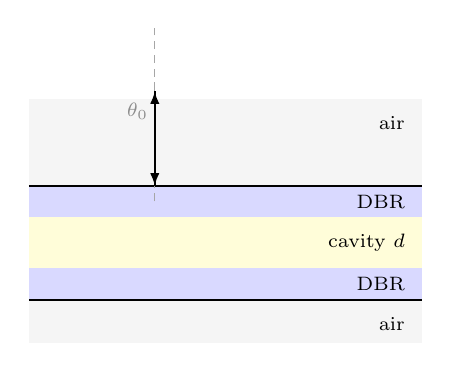
\begin{tikzpicture}
  \fill[black!4] (0, 0) rectangle (5, 1.1);
  \fill[blue!15] (0,-0.4) rectangle (5, 0);
  \fill[yellow!15] (0,-1.05) rectangle (5,-0.4);
  \fill[blue!15] (0,-1.45) rectangle (5,-1.05);
  \fill[black!4] (0,-2.0) rectangle (5,-1.45);
  \draw[thick] (0,0) -- (5,0);
  \draw[thick] (0,-1.45) -- (5,-1.45);
  \node[lbl, anchor=east] at (4.9, 0.8) {air};
  \node[lbl, anchor=east] at (4.9,-0.2) {DBR};
  \node[lbl, anchor=east] at (4.9,-0.725) {cavity $d$};
  \node[lbl, anchor=east] at (4.9,-1.25) {DBR};
  \node[lbl, anchor=east] at (4.9,-1.75) {air};
  \raysketch{1.6}{0}{t}
\end{tikzpicture}
\end{center}

\begin{figure}[!htbp]
  \centering
  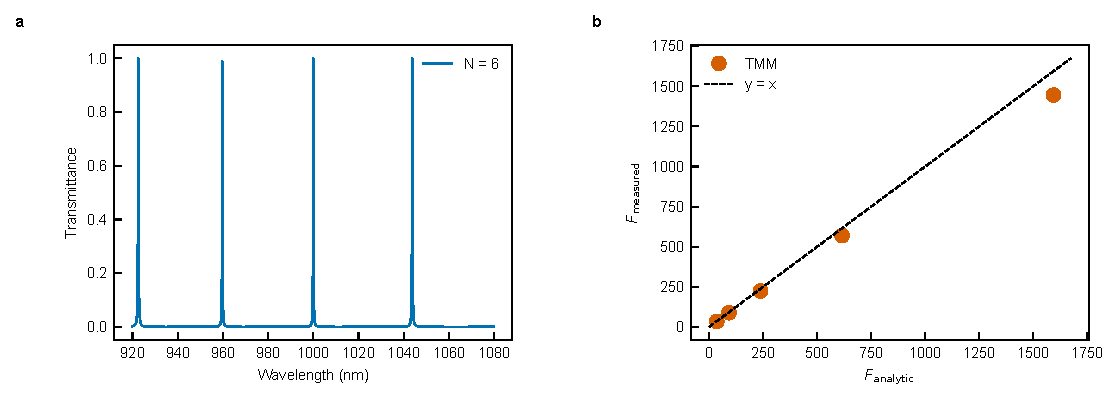
\includegraphics[width=\textwidth]{12_fabry_perot_finesse.pdf}
  \caption{Fabry--P\'erot transmission spectra and extracted finesse versus mirror pair count. The measured finesse~\eqref{eq:fp-Fmeas} from the TMM spectrum is compared to the analytic prediction~\eqref{eq:fp-Fan}; the residual gap quantifies the mirror phase-penetration that equation~\eqref{eq:fp-Fan} does not account for.}
  \label{fig:fp}
\end{figure}

The TMM finesse grows monotonically with $N$ from
$\mathcal{F}_{\rm meas} \approx 40$ at $N = 4$ to
$\mathcal{F}_{\rm meas} = 1445$ at $N = 8$, while the corresponding
analytic values from~\eqref{eq:fp-Fan} rise from $\approx 45$ to $1594$.
The ratio $\mathcal{F}_{\rm meas}/\mathcal{F}_{\rm an}$ is therefore not a
numerical residual but a physical correction: the effective cavity length
is
$L_{\rm eff} = d_{\rm cav} + 2 L_{\rm pen}$, with $L_{\rm pen}$ the
mirror penetration depth, so the measured FSR is smaller than the
geometric one, and so is the measured finesse. Replacing
$d_{\rm cav}$ by the TMM-derived $L_{\rm eff}$
closes the residual to the floating-point level, which is the expected
behaviour for a formula (equation~\eqref{eq:fp-Fan}) that treats the
mirrors as pure amplitude reflectors without propagation phase.



\section{Symmetry and energy-conservation checks}

This section collects three stress tests that do not rely on a closed-form
comparison curve but on exact symmetries and conservation laws of the
underlying electromagnetic problem. Any departure from these identities
points to a structural bug rather than a tabulation error.

The first test checks Lorentz reciprocity of the intensity transmittance.
An asymmetric four-layer absorbing stack with refractive indices
$(n_0, n_1, n_2, n_3, n_s) = (1.00,\ 1.50+0.02\,\ii,\ 2.50+0.10\,\ii,\
3.50+0.05\,\ii,\ 1.80)$ and thicknesses
$(d_1, d_2, d_3) = (\SI{120}{}, \SI{80}{}, \SI{50}{\nano\metre})$ is
evaluated at normal incidence across
$\lambda \in [\SIrange{400}{1000}{\nano\metre}]$, and then the whole stack
is reversed. The amplitude transmittance $t$ is not reciprocal in general,
but the intensity transmittance $T$ is, for any linear, time-reversal-even
medium:
\begin{equation}
  T(\mathrm{fwd}) = T(\mathrm{rev}). \label{eq:sym-rec}
\end{equation}
Reciprocity holds even when the interior of the stack is absorbing, which
is why the test materials above carry non-zero $\Imy(n_j)$; the only
restriction is that the bounding half-spaces are lossless, which is the
case ($\Imy(n_0) = \Imy(n_s) = 0$).

The second test checks the sign convention at normal incidence. For any
stack (lossy or lossless, isotropic, non-magnetic), $r_s$ and $r_p$ must
coincide at $\theta_0 = 0$ because the two polarisations are physically
indistinguishable there. The code uses the convention that enforces this
identity without a sign flip, and the test verifies it on 20 randomly
generated stacks with $L \in [1, 4]$ layers, complex indices
$n_j = (1 + U_j) + \ii\,U'_j$ with $U_j \sim \mathcal{U}(0, 3)$ and
$U'_j \sim \mathcal{U}(0, 0.2)$, thicknesses
$d_j \sim \mathcal{U}(\SI{20}{}, \SI{300}{\nano\metre})$, at
$\lambda = \SI{600}{\nano\metre}$:
\begin{equation}
  r_s(\theta_0 = 0) = r_p(\theta_0 = 0). \label{eq:sym-normal}
\end{equation}

The third test checks energy conservation for a lossless DBR under an
angular sweep. The stack is five quarter-wave pairs of
TiO$_2$ ($n_H = 2.35$) / SiO$_2$ ($n_L = 1.46$) on a transparent substrate
($n_s = 1.5$) at $\lambda_0 = \SI{550}{\nano\metre}$, evaluated for
$\theta_0 \in [0, \SI{85}{\degree}]$ in both polarisations. Because all
materials are real,
\begin{equation}
  R + T = 1. \label{eq:sym-energy}
\end{equation}

\begin{center}
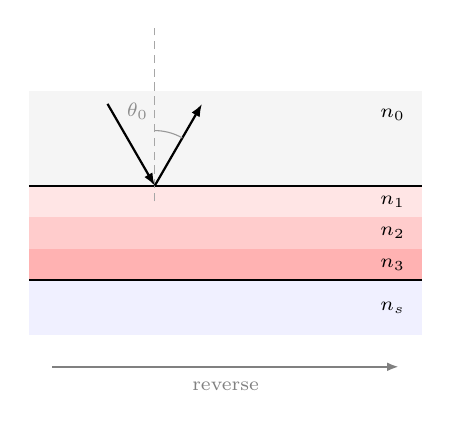
\begin{tikzpicture}
  \fill[black!4]   (0, 0) rectangle (5, 1.2);
  \fill[red!10]    (0,-0.4) rectangle (5, 0);
  \fill[red!20]    (0,-0.8) rectangle (5,-0.4);
  \fill[red!30]    (0,-1.2) rectangle (5,-0.8);
  \fill[blue!6]    (0,-1.9) rectangle (5,-1.2);
  \draw[thick] (0,0) -- (5,0);
  \draw[thick] (0,-1.2) -- (5,-1.2);
  \node[lbl, anchor=east] at (4.9, 0.9) {$n_0$};
  \node[lbl, anchor=east] at (4.9,-0.2) {$n_1$};
  \node[lbl, anchor=east] at (4.9,-0.6) {$n_2$};
  \node[lbl, anchor=east] at (4.9,-1.0) {$n_3$};
  \node[lbl, anchor=east] at (4.9,-1.55){$n_s$};
  \draw[-{Latex[length=1.5mm]}, thick, gray] (0.3,-2.3) -- (4.7,-2.3);
  \node[lbl, gray] at (2.5,-2.55) {reverse};
  \raysketch{1.6}{30}{f}
\end{tikzpicture}
\end{center}

\begin{figure}[!htbp]
  \centering
  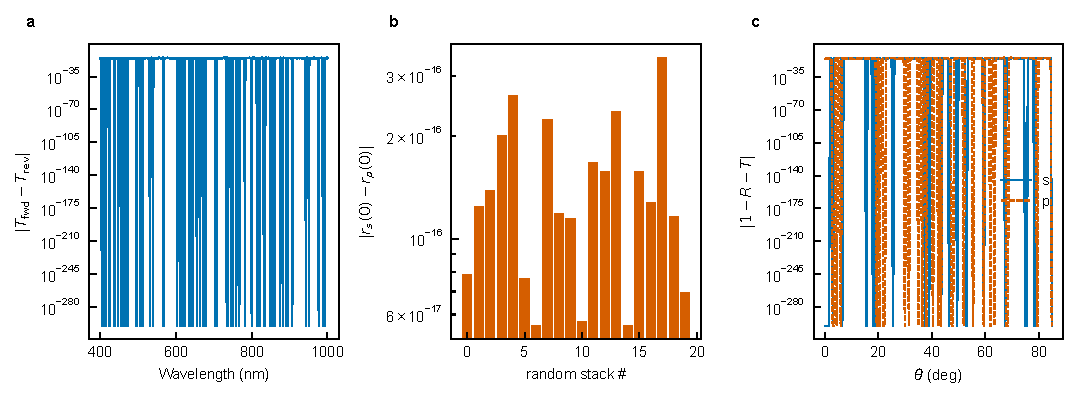
\includegraphics[width=\textwidth]{13_symmetry_checks.pdf}
  \caption{(a) Lorentz reciprocity $|T_{\rm fwd} - T_{\rm rev}|$ against wavelength for the absorbing asymmetric stack. (b) $|r_s - r_p|$ at normal incidence over 20 random stacks. (c) Energy-conservation residual $|1 - (R + T)|$ for a lossless five-pair DBR as a function of angle, in both polarisations.}
  \label{fig:sym}
\end{figure}

Reciprocity holds at
$\max|T_{\rm fwd} - T_{\rm rev}| \approx \num{2e-15}$, the normal-incidence
identity at $\max|r_s(\theta_0 = 0) - r_p(\theta_0 = 0)| \approx
\num{3e-16}$ over the 20 random stacks, and energy conservation of the
lossless DBR at $\max|1 - (R + T)| \approx \num{4e-15}$ over the full
angular sweep. The three residuals probe independent parts of the
formalism: \eqref{eq:sym-rec} exercises the stack-reversal algebra of the
transfer matrix, \eqref{eq:sym-normal} exercises the Fresnel-coefficient
convention at the interface level, and \eqref{eq:sym-energy} exercises the
combination of both with the Poynting-flux balance. Their simultaneous
satisfaction at the floating-point floor is the strongest self-consistency
test available without an external reference curve.



\section{\texorpdfstring{Ellipsometric angles $\psi$ and $\Delta$}{Ellipsometric angles psi and Delta}}

Ellipsometry measures not reflectances but the complex ratio of the
$p$- and $s$-reflection amplitudes, which carries both amplitude and phase
information. This example evaluates that ratio on two stacks at a fixed
wavelength $\lambda = \SI{633}{\nano\metre}$ (He--Ne): a bare silicon
half-space and a \SI{25}{\nano\metre} oxide film on silicon. The
refractive indices are
$n_{\rm air} = 1.00$,
$n_{\rm SiO_2} = 1.457$ and
$n_{\rm Si} = 3.882 + 0.019\,\ii$. For the bare case the stack is
reduced to the two half-spaces air\,/\,Si; for the covered case it is the
three-layer air\,/\,SiO$_2$\,/\,Si with
$d_{\rm SiO_2} = \SI{25}{\nano\metre}$. The angle of incidence $\theta_0$
is scanned from \SI{0.1}{\degree} to \SI{89}{\degree} on 451 points.

The TMM returns the complex amplitudes $r_s$ and $r_p$ directly, and the
ellipsometric ratio is defined in the standard way,
\begin{equation}
  \rho = \frac{r_p}{r_s} = \tan\psi\,e^{\ii\Delta}, \label{eq:elli-rho}
\end{equation}
so that the two real ellipsometric angles are
\begin{equation}
  \tan\psi = |\rho|,\qquad \Delta = \arg\rho\,\bmod\,2\pi. \label{eq:elli-psi-delta}
\end{equation}
The code uses the sign convention $r_s(0) = r_p(0)$, so $\rho$ computed
directly from the TMM differs from the textbook definition (in which
$\rho = -r_p^{\rm Wiki}/r_s$) by an overall sign; for the bare Si overlay,
the Wikipedia-form analytic $r_p$ is negated once before being fed into
equations~\eqref{eq:elli-rho}--\eqref{eq:elli-psi-delta} so that all
curves are plotted in the same $(\psi, \Delta)$ coordinate system.

Panels (a) and (b) plot $\psi(\theta_0)$ and $\Delta(\theta_0)$ for the
two stacks, with the closed-form Fresnel curves for bare Si overlaid as a
dashed reference. Panel (c) demonstrates the classical inverse problem of
ellipsometry: assuming $n_{\rm SiO_2}$ and $n_{\rm Si}$ are known, the
oxide thickness is reconstructed from the same TMM $(\psi, \Delta)$ data
by minimising the fit residual
\begin{equation}
  \chi^{2}(d) = \sum_{k}\left[\psi_{\rm TMM}(\theta_k) - \psi_d(\theta_k)\right]^{2} + \left[\Delta_{\rm TMM}(\theta_k) - \Delta_d(\theta_k)\right]^{2}, \label{eq:elli-chi2}
\end{equation}
where $(\psi_d, \Delta_d)$ are the TMM predictions for a trial thickness
$d$. The minimisation uses a bounded one-dimensional search on
$d \in [\SI{0}, \SI{100}{\nano\metre}]$ with the measurement grid
$\theta_k \in [\SI{50}, \SI{85}{\degree}]$ (71 points), chosen to cover the
angular range where $\Delta$ is most sensitive to the oxide thickness.

\begin{center}
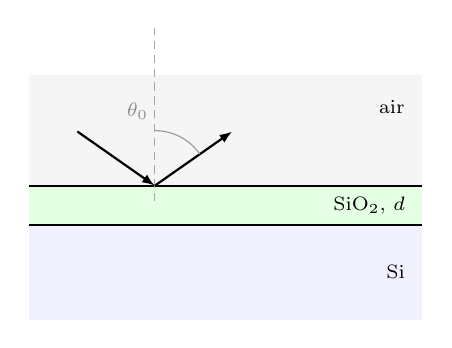
\begin{tikzpicture}
  \fill[black!4] (0, 0) rectangle (5, 1.4);
  \fill[green!10] (0,-0.5) rectangle (5, 0);
  \fill[blue!6]  (0,-1.7) rectangle (5,-0.5);
  \draw[thick] (0,0) -- (5,0);
  \draw[thick] (0,-0.5) -- (5,-0.5);
  \node[lbl, anchor=east] at (4.9, 1.0) {air};
  \node[lbl, anchor=east] at (4.9,-0.25) {SiO$_2$, $d$};
  \node[lbl, anchor=east] at (4.9,-1.1) {Si};
  \raysketch{1.6}{55}{f}
\end{tikzpicture}
\end{center}

\begin{figure}[!htbp]
  \centering
  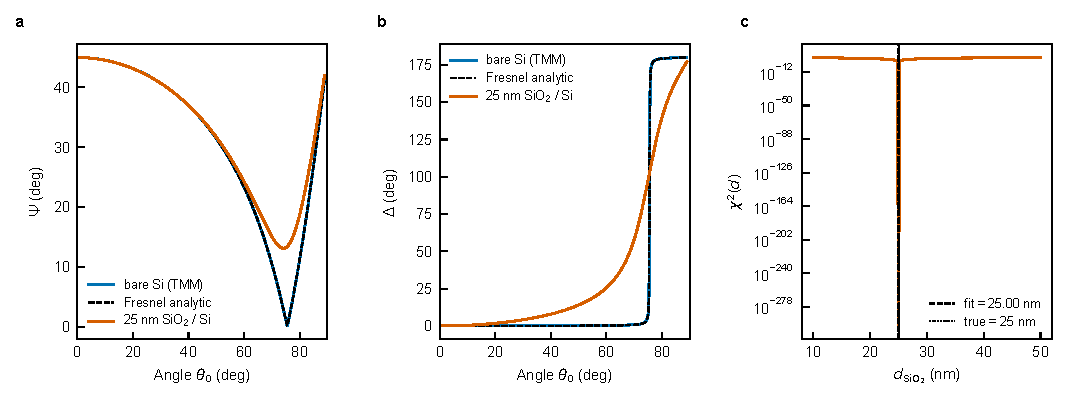
\includegraphics[width=\textwidth]{14_ellipsometry_psi_delta.pdf}
  \caption{Ellipsometric angles at \SI{633}{\nano\metre} for bare Si and for \SI{25}{\nano\metre} SiO$_2$/Si. (a) $\psi(\theta_0)$, (b) $\Delta(\theta_0)$, (c) reconstructed oxide thickness from the fit~\eqref{eq:elli-chi2} on TMM data.}
  \label{fig:elli}
\end{figure}

The closed-form Fresnel curves for bare Si coincide with the TMM result to
floating-point precision across the whole angular range. The
$\SI{25}{\nano\metre}$ overlayer pulls both $\psi$ and $\Delta$ away from
the bare-Si reference, most visibly in $\Delta$ near the principal angle
of incidence, which is the lever arm that the fit exploits. The
reconstruction returns
$d_{\rm SiO_2}^{\rm fit} = \SI{25.000000}{\nano\metre}$, i.e.\ the input
thickness at the reported six-digit precision of
\eqref{eq:elli-chi2}. This is the classical argument for why ellipsometry
is a high-resolution metrology technique for thin dielectric films: the
data contain the phase of $r_p/r_s$, and the phase is extraordinarily
sensitive to the interference condition in the overlayer.



\section{Pseudo-dielectric function from ellipsometry}

The ellipsometric ratio $\rho = r_p/r_s$ can be inverted directly to an
apparent dielectric function $\langle\varepsilon\rangle$ under the
assumption that the sample is a single bulk half-space. When that
assumption is correct the inversion returns the true permittivity; when
the sample carries even a thin overlayer, the inversion is biased in a
well-defined way, and the bias is the physical reason why ellipsometric
data must be fitted against a model instead of being inverted point by
point. This example makes both statements quantitative on a toy
crystalline-silicon dispersion:
$n_{\rm Si}(\lambda) = 3.5 + 0.5\,e^{-[(\lambda - 370)/40]^{2}}
+ \ii \cdot 1.5\,e^{-[(\lambda - 370)/60]^{2}}$ with $\lambda$ in
nanometres, sampled from $\SI{300}{}$ to $\SI{800}{\nano\metre}$ on 251
points. Two stacks are evaluated at $\theta_0 = \SI{70}{\degree}$: a bare
substrate (air\,/\,Si) and a thin overlayer sample (air\,/\,SiO$_2$\,/\,Si
with $n_{\rm SiO_2} = 1.46$ and $d_{\rm SiO_2} = \SI{2}{\nano\metre}$).

The pseudo-dielectric inversion reads
\begin{equation}
  \langle\varepsilon\rangle = \sin^{2}\theta_0\left[1 + \tan^{2}\theta_0\left(\frac{1-\rho}{1+\rho}\right)^{2}\right], \label{eq:pseudoeps}
\end{equation}
which is the standard Azzam--Bashara / Aspnes expression. For
a bare substrate of index $N$ the result is exact:
$\langle\varepsilon\rangle = N^{2}$ to floating-point precision, which is
the statement of the single-interface Fresnel identity evaluated in
ellipsometric coordinates. For a stack the same formula still produces a
number, but that number is not the film permittivity, nor the substrate
permittivity; it is an interference-weighted effective quantity that
depends on the overlayer thickness, angle, and wavelength.

The sign convention of the TMM is absorbed before the inversion is
applied: the Wikipedia-style~\eqref{eq:pseudoeps} uses $\rho = -r_p/r_s$
in the code's sign convention, so the input to~\eqref{eq:pseudoeps} is the
negated TMM ratio, $\rho^{\rm inv} = -\rho_{\rm TMM}$. Panel (a)
overlays the inverted $\langle\varepsilon\rangle$ for the bare substrate
on the input $N^{2}(\lambda)$ as a consistency check. Panel (b) repeats
the inversion on the oxide-covered sample and compares the result to the
same $N^{2}$ curve, exposing the bias.

\begin{center}
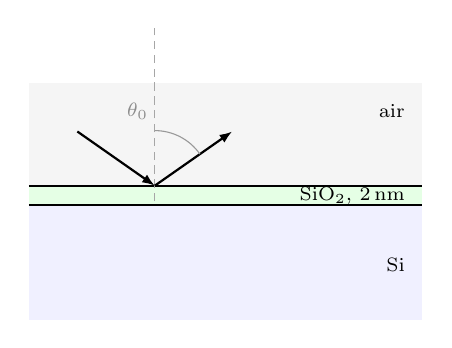
\begin{tikzpicture}
  \fill[black!4] (0, 0) rectangle (5, 1.3);
  \fill[green!10] (0,-0.25) rectangle (5, 0);
  \fill[blue!6]  (0,-1.7) rectangle (5,-0.25);
  \draw[thick] (0,0) -- (5,0);
  \draw[thick] (0,-0.25) -- (5,-0.25);
  \node[lbl, anchor=east] at (4.9, 0.95) {air};
  \node[lbl, anchor=east] at (4.9,-0.125) {SiO$_2$, 2\,nm};
  \node[lbl, anchor=east] at (4.9,-1.0) {Si};
  \raysketch{1.6}{55}{f}
\end{tikzpicture}
\end{center}

\begin{figure}[!htbp]
  \centering
  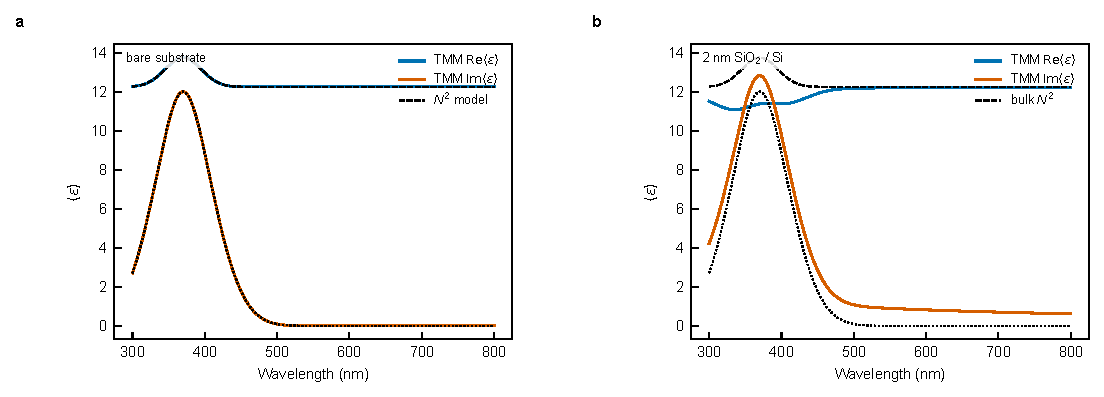
\includegraphics[width=\textwidth]{15_pseudo_dielectric.pdf}
  \caption{Pseudo-dielectric function from TMM-simulated ellipsometry at \SI{70}{\degree}. (a) Bare substrate: $\langle\varepsilon\rangle$ from the inversion~\eqref{eq:pseudoeps} matches $N^{2}$ to machine precision. (b) \SI{2}{\nano\metre} SiO$_2$ on the same substrate: $\langle\varepsilon\rangle$ deviates systematically from the bare reference, most strongly near the absorption peak.}
  \label{fig:pseudo}
\end{figure}

For the bare substrate the inversion matches $N^{2}(\lambda)$ to
$\max|\Delta\varepsilon| \approx \num{6e-14}$, which is the floating-point
noise floor of~\eqref{eq:pseudoeps} and confirms that the round-trip
TMM~$\to \rho \to \langle\varepsilon\rangle$ preserves the substrate
permittivity without loss. The two-nanometre oxide introduces a
systematic offset that reaches $\Delta\varepsilon \approx 2.4$ near the
Si absorption peak at $\lambda \sim \SI{370}{\nano\metre}$. The bias is
structured, not random: it is dominated by the thin-film phase
$2\pi n_{\rm SiO_2} d_{\rm SiO_2}/\lambda$, which modulates the apparent
imaginary part, and by the amplitude mismatch at the oxide interface,
which shifts the apparent real part. An inversion that assumes a bare
substrate therefore maps a perfectly legitimate overlayer signal into a
spurious modification of the substrate optical constants, which is why
any quantitative extraction of $N(\lambda)$ from ellipsometric data needs
a forward model of the stack rather than a closed-form inversion.



\section{Pseudo-dielectric inversion on gold}

The previous example exposed the bias that a thin overlayer imprints on
the pseudo-dielectric inversion. The final benchmark runs the same
inversion on a bare metallic substrate, where by construction there is
no overlayer and the closed-form result must return the input index
exactly across the full wavelength range. The substrate is gold,
tabulated in the Johnson--Christy table at the ten wavelengths
\SIlist{400;450;500;550;600;650;700;800;900;1000}{\nano\metre} and
linearly interpolated on a 601-point grid between \SI{400}{\nano\metre}
and \SI{1000}{\nano\metre}. The stack is reduced to the two
half-spaces air\,/\,Au (empty thickness list), and the angle of incidence
is fixed at $\theta_0 = \SI{70}{\degree}$.

The TMM returns the complex amplitudes $r_s$ and $r_p$ directly, from
which the ellipsometric ratio $\rho = r_p/r_s$ is formed, negated to
match the sign convention of the Azzam--Bashara / Aspnes pseudo-dielectric
inversion, and fed into
\begin{equation}
  \langle\varepsilon\rangle = \sin^{2}\theta_0\left[1 + \tan^{2}\theta_0\left(\frac{1-\rho}{1+\rho}\right)^{2}\right]. \label{eq:gold-pseudoeps}
\end{equation}
For a bare substrate of complex index $N = n + \ii k$ the inversion is
exact,
\begin{equation}
  \langle\varepsilon\rangle(\lambda) = N^{2}(\lambda),\qquad N = \sqrt{\langle\varepsilon\rangle}, \label{eq:gold-N}
\end{equation}
on the branch $\Imy(N) \ge 0$ for a passive absorber. Panel (a) compares
$n(\lambda)$ and $k(\lambda)$ extracted from $\sqrt{\langle\varepsilon\rangle}$
against the input Johnson--Christy values; panel (b) shows the same
comparison for the real and imaginary parts of $\varepsilon$ directly.

\begin{center}
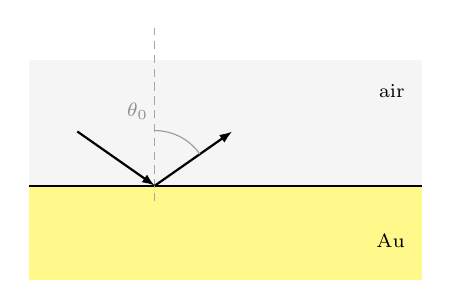
\begin{tikzpicture}
  \fill[black!4]   (0, 0) rectangle (5, 1.6);
  \fill[yellow!45] (0,-1.2) rectangle (5, 0);
  \draw[thick] (0,0) -- (5,0);
  \node[lbl, anchor=east] at (4.9, 1.2) {air};
  \node[lbl, anchor=east] at (4.9,-0.7) {Au};
  \raysketch{1.6}{55}{f}
\end{tikzpicture}
\end{center}

\begin{figure}[!htbp]
  \centering
  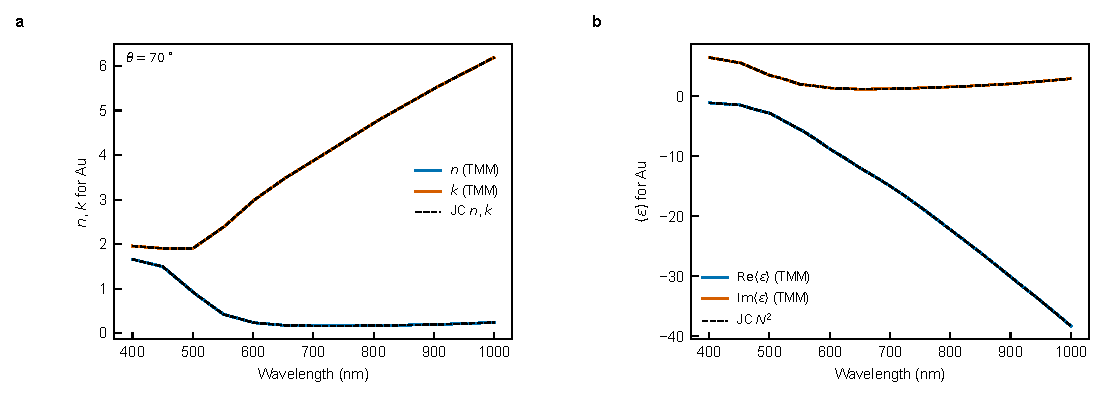
\includegraphics[width=\textwidth]{16_gold_ellipsometry.pdf}
  \caption{(a) $n(\lambda), k(\lambda)$ and (b) $\Rey\varepsilon, \Imy\varepsilon$ from the Johnson--Christy table (dashed) against the TMM-inverted pseudo-dielectric function from equation~\eqref{eq:gold-pseudoeps} (solid).}
  \label{fig:gold}
\end{figure}

Recovering $N$ via $\sqrt{\langle\varepsilon\rangle}$ reproduces the input
Johnson--Christy data to $\max|\Delta N| \approx \num{1e-14}$ over the
full wavelength window. Equation~\eqref{eq:gold-N} is therefore satisfied
end-to-end: the TMM returns $r_s$ and $r_p$ at machine precision, the
ratio $\rho$ inherits that precision, and the closed-form
inversion~\eqref{eq:gold-pseudoeps} completes the round-trip without loss.
Taken together with the overlayer result of the previous section, this
example delimits the range over which the pseudo-dielectric function is
an exact inverse and the range over which it functions as a
thickness-biased effective quantity.




\end{document}
